%*******************************************************************************
%*********************************** First Chapter *****************************
%*******************************************************************************

\chapter{Event Detection Using Segment-based Feature Representation}  %Title of the First Chapter
\label{chapter3}
%\setlength{\epigraphrule}{0pt}
\epigraph{\textit{Concentrate all your thoughts upon the work at hand. The sun's rays do not burn until brought to a focus.}}{ -- Alexander Graham Bell}

\ifpdf
    \graphicspath{{Chapter3/Figs/Raster/}{Chapter3/Figs/PDF/}{Chapter3/Figs/}}
\else
    \graphicspath{{Chapter3/Figs/Vector/}{Chapter3/Figs/}}
\fi


\section{Introduction}
\label{introduction:1}
Multimedia Event Detection (MED) is a challenging task in TREC Video Retrieval Evaluation (TRECVID)\footnote{http://trecvid.nist.gov/}. The task is defined as follow: given a collection of test videos and a list of test events, indicate whether each of the test events is present in each of the test videos. The aim of MED is to develop systems that can automatically find video containing any event of interest, assuming only a limited number of training exemplars are given.

%\begin{figure}
%	\centering
%	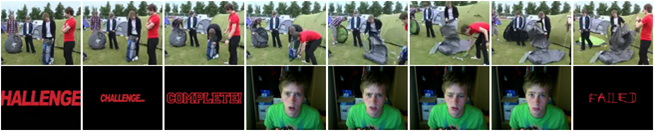
\includegraphics[width=1\textwidth]{teaser_image.eps}
%	\caption{(a) Example video for "making a sandwich" event: the related segment appears after a self-cam segment (unrelated); (b) example video for "grooming an animal" event: related segment is sandwiched between two unrelated segments. This kind of video is popular in realistic video datasets like MED. The frames with a red outlined box are examples of the extracted keyframes when using a keyframe-based approach, which suffers from both noise and missed extraction.}
%	\label{teaser_image}
%\end{figure}


The need for such MED systems is rising because a massive number of videos are produced every day. For example, more than 3 million hours of video are uploaded and over 3 billion hours of video are watched each month on YouTube\footnote{http://www.youtube.com/t/press\_statistics}, the most popular video sharing website. What is needed are the tools for automatically processing the video content and looking for the presence of a complex event in such unconstrained capturing videos. Automatic detection of complex events has great potential for many applications in the field of web video indexing and retrieval. In practice, a viewer may only want to watch goal scenes in a long football video, a housewife may need to search for videos that teach her how to make a cake, a handyman may look for how to repair an appliance, or a TV program manager may want to remove violent scenes in a film before it is aired.

However, detecting events in multimedia videos is a difficult task due to both the large content variation and uncontrolled capturing conditions. The video content is extremely diverse even in a same event class. The genres of video are also very varied, such as interviews, home videos, and tutorials. Moreover, the number of events is expected to be extensive for large scale processing. Each event, in its turn, can involve a number of objects and actions in a particular setting (indoors, outdoors, etc). Furthermore, multimedia videos are typically recorded under uncontrolled conditions such as different lighting, viewpoints, occlusions, complicated camera motions and cinematic effects. Therefore, it is very hard to model and detect of multimedia events.

The most straightforward approach toward building a large scale event detection system is using a bag-of-words (BoW) model \cite{Csurka04visualcategorization}. There are two types of BoW representations that are used for MED: BoW representation at the keyframe level and BoW representation at the video level. The first method is employed for still image features where the keyframes are often extracted at a fixed interval. The second method is employed for motion features where moving patterns from the entire video are extracted. These methods are respectively referred to as keyframe-based \cite{trecvid10:IBM,trecvid10:cuucf,DBLP:conf/trecvid/MatsuoN10} and video-based \cite{trecvid10:IBM,trecvid10:cuucf} in this chapter. Although these methods can obtain reasonable results, they all suffer from severe limitations. For the keyframe-based approach, temporal information is not incorporated in the model. Moreover, it is possible that important keyframes are missed extraction. Extracting more keyframes can tackle this problem but the scalability is also a problem for concern. On the other hand, the video-based approach is most likely to suffer from noise. We found that the video length is very different from video to video (even from videos of the same event class). In addition, the clues to determine an event may appear within a small segment of the entire video. Thus, comparing the BoW representation of two videos is unreliable because it may contain unrelated information. Figure \ref{c1_uncontrolled} illustrates these limitations for both approaches. 

In this chapter, we propose using a segment-based approach to overcome the limitations of both the keyframe-based and video-based approaches. The basic idea is to examine shorter segments instead of using the representative frames or entire video. We can reduce the amount of unrelated information in the final representation, while still benefiting from the temporal information by dividing a video into segments. In particular, we investigate two methods to cut a video into segments. The first method is called uniform sampling, where every segment has an equal length. We choose different segment lengths and use two types of sampling: non-overlapping and overlapping. The overlapped configuration is used to test the influence of dense segment sampling. The second method divides the video based on the shot boundary detection to take into account the boundary information of each segment. Once segments are extracted, we use dense trajectories, a state-of-the-art motion feature proposed by Wang \cite{wang:2011:inria-00583818:1}, for the feature extraction. After that, a BoW model is employed for the feature representation. The experimental results on TRECVID MED 2010 and TRECVID MED 2011 showed the improvement of the segment-based approach over the video-based approach. Moreover, a better performance can be obtained by using the overlapping sampling strategy. 

The rest of this chapter is organized as follows. Section \ref{relatedwork:1} introduces the related work. Section \ref{sec:1} gives an overview of the dense trajectory motion feature and our segment-based approach. The experimental setup including an introduction to the benchmark dataset and the evaluation method are presented in Section \ref{experimentalsetup}. Then, in Section \ref{experimentalresult}, we present and analyze our experimental results. Detailed discussions of these results are presented in Section \ref{discussion}. Finally, Section \ref{c3_conclusion} concludes this work with discussions on our future work. 

\section{Related Work}
\label{relatedwork:1}
Challenges began from TRECVID 2010\footnote{www.nist.gov/itl/iad/mig/med10.cfm}, and Multimedia Event Detection has drawn the attention of many researchers. Seven teams participated in the debut challenge and 19 teams participated the following year (MED 2011). Many MED systems have been built and different strategies have been used for the event detection system.

Columbia University (CU) team achieved the best result in TRECVID MED 2010. Their success greatly influenced later MED systems. In their paper \cite{trecvid10:cuucf}, they answered two important questions. The first question was, "What kind of feature is more effective for multimedia event detection?". The second one was, "Are features from different feature modalities (e.g., audio and visual) complementary for event detection?". Different kinds of features have been studied, such as SIFT \cite{Lowe:2004} for the image feature, STIP \cite{Laptev:2005:SIP} for the motion feature and MFCC (Mel-frequency cepstral coefficients \cite{Lee1998MFCC}) for the audio feature to answer the first question. In general, the STIP motion feature is the best single feature for MED. However, the system should combine strong complementary features from multiple modalities (both visual and audio) in order to achieve better results. 

The IBM team \cite{trecvid10:IBM} achieved the runner-up MED system in TRECVID 2010. They incorporated information from a wide range of static and dynamic visual features to build their baseline detection system. For the static features, they used the local SIFT \cite{Lowe:2004}, GIST \cite{DBLP:livaT01} descriptors and various global features such as Color Histogram, Color Correlogram, Color Moments, Wavelet Texture, etc. They used the STIP \cite{Laptev:2005:SIP} feature with a combined HOG-HOF \cite{Laptev08CVPR} descriptor for the dynamic feature.

The Nikon MED 2010 system \cite{DBLP:conf/trecvid/MatsuoN10} is also a remarkable system due to its simple but effective solution. They built a MED system based on the assumption that a small number of images in a given video contain enough information for event detection. Thus, they reduced the event detection task to the classification problem for a set of images, called keyframes. However, keyframe extraction is based on a scene cut detection technique \cite{Guimaraes:2003} that is less reliable in realistic videos. Moreover, the scene length is not consistent, which may affect the detection performance.

The BBN Viser system \cite{NIST-TRECVID11:BBN-DVMM} achieved the best performance at TRECVID MED 2011. Their success confirmed the effectiveness of the multiple modalities approach for multimedia event detection. In their work, they further investigated the performance of the appearance features (e.g., SIFT \cite{Lowe:2004}), color feature (e.g. RGB-SIFT \cite{vandeSandeTPAMI2010}), and motion (e.g., STIP \cite{Laptev:2005:SIP}), and also MFCC \cite{Lee1998MFCC} based audio features. Different kinds of fusion strategies have been explored, from which the novel non-parametric fusion strategy based on a video specific weighted average fusion has shown promising results.

In general, most systems used the multiple modalities approach to exploit different visual cues to build their baseline detection systems. Static image characteristics are extracted from frames within provided videos. Colombia University's results \cite{trecvid10:cuucf} suggest that methods for exploiting semantic content from web images, such as \cite{duan2012exploiting} and \cite{trecvid10:cuucf}, are not effective for multimedia event detection. For motion characteristics, most systems employed the popular STIP proposed by Laptev in \cite{Laptev:2005:SIP} for detecting complex actions. Other systems also took into account the HOG3D \cite{Klaser08BMVC} and MoSIFT \cite{Chen_mosift} motion features. All these systems used a video-based approach for the motion features, i.e., the motion features are extracted from the entire video. IBM's MED system \cite{trecvid10:IBM} also applied the video-based approach but the video was downsampled to five frames per second. One drawback of this video-based approach is that it may encode unrelated information in the final video representation. In a long video, the event information may happen during a small segment, and the information from the other segments tends to be noisy. That is why it is important to localize the event segment (i.e., where the event happens). This problem has been thoroughly investigated by Yuan et. al. \cite{Yuan2011PAMI}. Yuan proposed using a spatio-temporal branch-and-bound search to quickly localize the volume where an action might happen. In \cite{xu2008video}, Xu proposed a method to find optimal frame alignment in the
temporal dimension to recognize events in broadcast news. In \cite{duan2012visual}, a transfer learning method is proposed to recognize simple action events. However, these works are not applicable for complex actions in multimedia event videos.

Different from other approaches, we use a segment-based approach for the event detection. We did not try to localize the event volume like Yuan in \cite{Yuan2011PAMI}. In a simpler way, we use a uniform sampling with different segment lengths for our evaluation. We also investigate the benefit of using the shot boundary detection technique in \cite{Guimaraes:2003} for dividing video into segments. Moreover, an overlapped segment sampling strategy is also considered for a denser sampling. To the best of our knowledge, no MED system has previously used this approach. We evaluate its performance using the dense trajectories motion feature that was recently proposed by Wang in \cite{wang:2011:inria-00583818:1}. The dense trajectories feature has achieved state-of-the-art performances for various video datasets, including challenging datasets like Youtube Action \cite{liu2009recognizing} and UCF Sports \cite{Rodriguez2008}. In TRECVID MED 2012, the dense trajectories feature was also widely used by top performance systems such as AXES \cite{oneata:hal-00746874}, and BBNVISER \cite{NIST-TRECVID12:BBN-DVMM}. We use the popular ``bag-of-words'' model in \cite{Csurka04visualcategorization} as our feature representation technique. Finally, we use a Support Vector Machine (SVM) classifier for the training and testing steps. \index{segment-based}

\section{Dense Trajectories and Segment-based Approach}
\label{sec:1}
We introduce the dense trajectory motion feature proposed by Wang in \cite{wang:2011:inria-00583818:1} in this section. We additionally briefly review the trajectory extraction and description method. A detailed calculation of all the related feature descriptors, especially for Motion Boundary Histogram, is also presented. Our segment-based approach for motion features is introduced at the end of this section.

\subsection{Dense Trajectories} \index{dense trajectories}
\label{subsec:1}
Trajectories are obtained by tracking the densely sampled points using the optical flow fields. First, the feature points are sampled on a grid with a step size of 5 pixels and at multiple scales spaced by a factor of 1/$\sqrt{2}$. Then, the feature points are separately tracked in each scale. Each point $P_{t} = (x_{t}, y_{t})$ at frame \textit{t} is tracked to the next frame \textit{t+1} by using median filtering in a dense optical flow field $\omega$ = ($u_{t}$, $v_{t}$):
\begin{equation}
P_{t+1}=(x_{t+1}, y_{t+1})=(x_{t},y_{t}) + (M*\omega)|_{(\bar{x}_{t},\bar{y}_{t})},
\end{equation}
where \textit{M} is the median filter, and $(\bar{x}_{t},\bar{y}_{t})$ is the rounded position of $(x_{t}, y_{t})$.

After extracting a trajectory, two kinds of feature descriptors are adopted: a trajectory shape descriptor and a trajectory-aligned descriptor.

\textit{Trajectory shape descriptor:} The trajectory shape descriptor is the simplest one for representing an extracted trajectory. It is defined based on the displacement vectors. Given a trajectory of length L, its shape is described by the sequence S = ($\Delta P_{t}$ ,..., $\Delta P_{t+L-1}$), where $\Delta P_{t}$ = $P_{t+1} - P_{t}$ = ($x_{t+1} - x_{t}$, $y_{t+1} - y_{t}$). The resulting vector is then normalized by the sum of the magnitudes of the displacement vectors:
\begin{equation}
S'=\dfrac{(\Delta P_{t},...,\Delta P_{t+L-1})}{\sum_{j=t}^{t+L-1} \|\Delta P_{j}\|}
\end{equation}
\textit{Trajectory-aligned descriptor:} More complex descriptors can be computed within a space-time volume around the trajectory. The size of the volume is NxN spatial pixels and L temporal frames. This volume is further divided into a $n_{\sigma}$ x $n_{\sigma}$ x $n_{\tau}$ grid to encode the spatial-temporal information between the features. The default settings for these parameters are N = 32 pixels, L = 15 frames, $n_{\sigma}$ = 2, and $n_{\tau}$ = 3. The features are separately calculated and aggregated in each region. Finally, the features in all regions are concatenated to form a single representation for the trajectory. Three kinds of descriptors have been employed for representing trajectory following this design: The Histogram of Oriented Gradient (HOG), which was proposed by Dalal et al. in \cite{DBLP:DalalT05} for object detection, The Histogram of Optical Flow (HOF), which was used by Laptev in \cite{Laptev08CVPR} for human action recognition, and the Motion Boundary Histogram (MBH). The MBH descriptor was also proposed by Dalal et al.~\cite{Dalal06ECCV} for human detection, where the derivatives are computed separately for the horizontal and vertical components of the optical flow $I_{\omega}$ = ($I_{x}$, $I_{y}$). The spatial derivatives are computed for each component of the optical flow field $I_{x}$ and $I_{y}$ independently. After that, the orientation information is quantized into histogram, similarly to that for the HOG descriptor (8-bin histogram for each component). Finally, these two histograms are normalized separately with the $L_{2}$ norm and concatenated together to form the final representation. Since the MBH represents the gradient of the optical flow, constant motion information is suppressed and only the information concerning the changes in the flow field (i.e., motion boundaries) is kept.

According to the author \cite{wang:2011:inria-00583818:1}, the MBH descriptor is the best feature descriptor for dense trajectories. One interesting property of the MBH is that it can cancel out camera motion. That is why it shows significant improvement on realistic action recognition dataset compared to other trajectory descriptors. We only use the MBH descriptor in this study to test the performance of our proposed segment-based method.

\subsection{Segment-based Approach for Motion Feature}
\label{subsec:4}
\begin{figure}
	\centering
	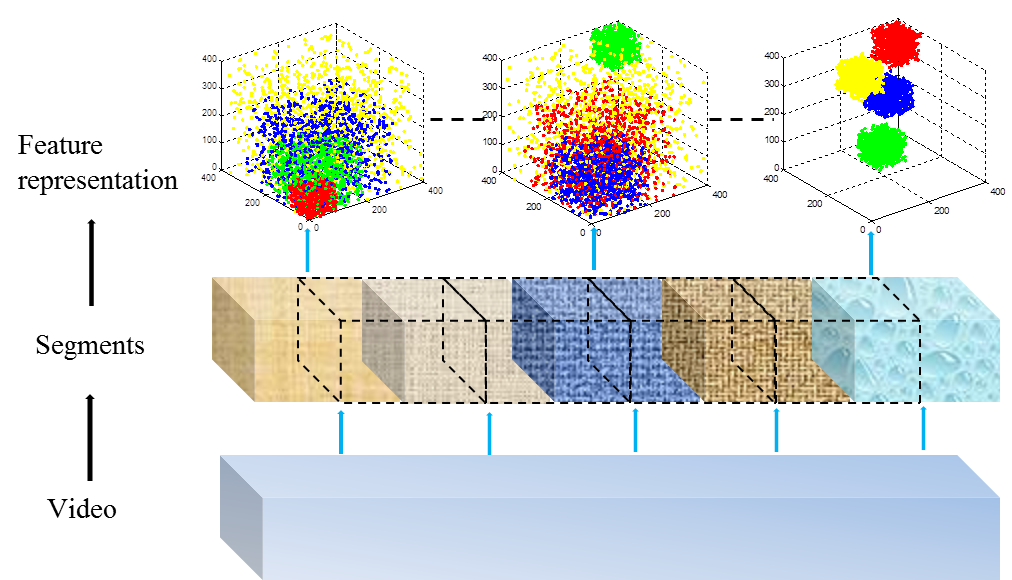
\includegraphics[width=1\textwidth]{segment_based.eps}
	\caption{Illustration of our segment-based approach. The original video is divided into segments by using non-overlapping and overlapping sampling (overlapped segment examples are drawn in dashes). After that, the feature representation is separately calculated for each segment. This figure is best viewed in color.}
	\label{segmentbased}
\end{figure}

Our proposed segment-based approach is as follows. At first, the video is divided into fixed length segments. We choose different segment lengths to pick the optimal one. In particular, we choose segment lengths of 30, 60, 90, 120, 200 and 400 seconds. The lengths of 120 and 60 seconds are respectively close to the mean (115 s) and geometric mean (72 s) length of the training dataset. The geometric mean value is also considered because it can eliminate the influence of outline cases, i.e., videos of exceptionally long durations. After that, the dense trajectory features are extracted from the entire segment. A "bag-of-words" approach is used to generate the final representation for each segment from the raw trajectory features (Fig. \ref{segmentbased}).

For the previous segment-based approach, a video is divided into continuous segments. This means information about the semantic boundary of a segment is not taken into account. However, this information is important because it keeps the semantic meaning of each segment. The simplest way to overcome this drawback is to use a denser sampling such as the overlapped segments. We use an overlapping strategy for the same segment length as in the non-overlapping experiments. In practice, we use uniform segment sampling with 50\% of overlapping. This means the number of segments will be doubled for each overlapping experiment.

Another way to extract segments with boundary information is to employ a shot boundary detection technique. For a fast implementation, we use the algorithm proposed in \cite{Guimaraes:2003}. This technique is also used in the Nikon 2010 MED system \cite{DBLP:conf/trecvid/MatsuoN10}. Basically, at first, this method constructs a space-time image from the input video. We can sample points or calculate the color histogram for each frame to construct the space-time image. This will reduce the 2D frame image to the space dimension of the space-time image. The time dimension is the number of frames of the video. The Canny edge detection algorithm is used to detect the vertical lines after attaining the space-time image. Each detected vertical line is considered as a scene cut. The method in \cite{Guimaraes:2003} also proposed solutions for other kinds of scene transitions such as a fade or wide. However, from our previous study, this method showed poor results in these cases. Thus, we only adopted the scene cut detection algorithm. Each detected scene cut is considered a segment in our experiments. \index{shot boundary detection}

Our proposed segment-based approach is compared with the video-based one. Actually, when the segment length is long enough, it becomes the entire video. In that case, we can consider the video-based approach a special type of segment-based approach.
\section{Experimental Setup}
\label{experimentalsetup}
\subsection{Dataset}
\label{experimentalsetup:1}
We tested our method on TRECVID MED 2010 and TRECVID MED 2011 datasets. An event kit is provided with the definitions and textual descriptions for all the events for each dataset. The first dataset contains 3,468 videos, including 1,744 videos for training and 1,724 video clips for testing, containing a total of more than 110 video hours. In TRECVID MED 2010, there are 3 events classes: assembling a shelter, batting in a run, and making a cake. The TRECVID MED 2011 dataset defined the 15 event classes listed in Table \ref{med11}. The first five events (E001-E005) are used for training and validation and the last 10 events (E006-E015) are used for testing. It comprises of over 45,000 video clips for a total of 1,400 hours of video data. All the video clips are divided into three sets: event collection (2392 video clips), development collection (10198 video clips), and test collection (31,800 video clips). It is worth noting that these two datasets contain a major number of background video clips, i.e., video clips that do not belong to any event. The number of positive videos in the event collection is also listed in Table \ref{med11}.

% Table generated by Excel2LaTeX from sheet 'Sheet1'
\begin{table}[!h]
	\renewcommand{\arraystretch}{1.3}
	\centering
	\caption{List of events and its number of positive samples in event collection set of MED 2011 dataset.}
	\begin{tabular}{|c|l|c|}
		\toprule
		Event ID & Event Name & \#Pos videos \\
		\midrule
		E001  & Attempting a board trick & 173 \\
		\midrule
		E002  & Feeding an animal & 168 \\
		\midrule
		E003  & Landing a fish & 152 \\
		\midrule
		E004  & Wedding ceremony & 163 \\
		\midrule
		E005  & Working on a woodworking project & 159 \\
		\midrule
		E006  & Birthday party & 221 \\
		\midrule
		E007  & Changing a vehicle tire & 119 \\
		\midrule
		E008  & Flashmob gathering & 191 \\
		\midrule
		E009  & Getting a vehicle unstuck & 151 \\
		\midrule
		E010  & Grooming an animal & 143 \\
		\midrule
		E011  & Making a sandwich & 186 \\
		\midrule
		E012  & Parade & 171 \\
		\midrule
		E013  & Parkour & 134 \\
		\midrule
		E014  & Repairing an appliance & 137 \\
		\midrule
		E015  & Working on a sewing project & 124 \\
		\bottomrule
	\end{tabular}%
	\label{med11}%
\end{table}%

\subsection{Evaluation Method}
\label{experimentalsetup:2}
%
Figure \ref{framework} shows our evaluation framework for the motion features. We conducted experiments using the proposed segment-based approach and the video-based approach for comparison. We use the library published online by the author\footnote{http://lear.inrialpes.fr/people/wang/dense\_trajectories} to extract dense trajectory feature. The source code is customized for pipeline processing using only an MBH descriptor to save computing time but other parameters are set to default. Due to the large number of features produced when using the dense sampling strategy, we use the "bag-of-words" approach to generate the features for each segment. At first, we randomly select 1,000,000 dense trajectories for clustering to form a codebook of 4000 visual codewords. After that, the frequency histogram of the visual words is computed over the videos/segments to generate the final feature vector. We also adopt the soft assignment weighting scheme, which was initially proposed by Jiang in \cite{Jiang:2007:TOB}, to improve the performance of the ``bag-of-words'' approach.
\begin{figure}
	\centering
	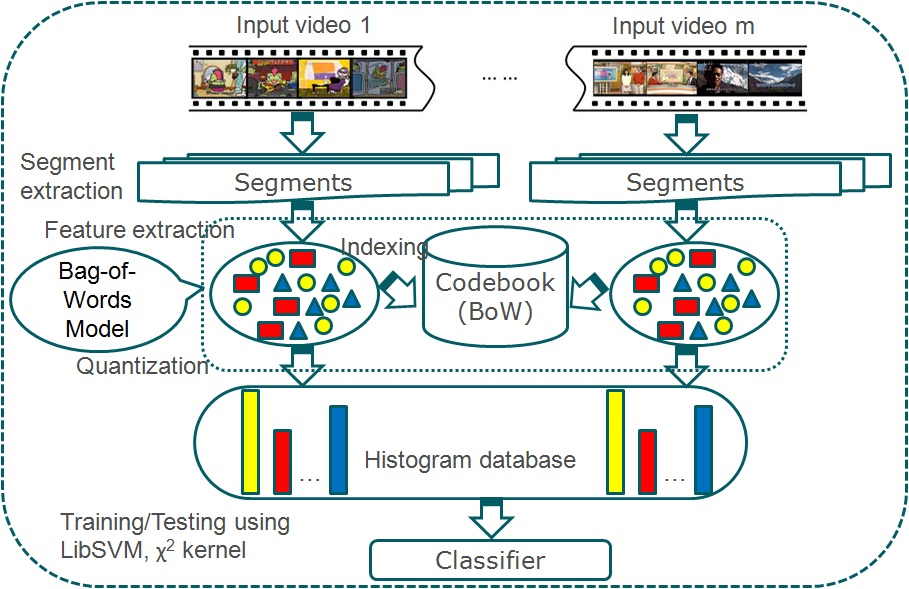
\includegraphics[width=1\textwidth]{baseline_framework.jpg}
	\caption{Evaluation framework for our baseline MED system}
	\label{framework}
\end{figure}

Once all the features are extracted, we use the popular Support Vector Machine (SVM) for the classification. In particular, we use the LibSVM library available online\footnote{http://www.csie.ntu.edu.tw/{\textasciitilde}cjlin/libsvm/} and adopt the one-vs.-rest scheme for multi-class classification. We annotate the data in the following way to prepare it for the classifier. All the videos/segments from positive videos are considered positive samples, and the remaining videos/segments (in the development set) are chosen as the negative samples. For testing purposes, we also use the LibSVM to predict the scores of the videos/segments in each testing video. The score of a video is defined as the largest score among its videos/segments. This score indicates how likely a video belongs to an event class.

\section{Experimental Result}
\label{experimentalresult}

\begin{table*}
	\renewcommand{\arraystretch}{1.3}
	\caption{Results on the MED 2010 dataset using non-overlapping sampling.}
	\label{t_med10_nonoverlapping}
	\centering
	\begin{tabular}{|l|cccccc|c|}
		\toprule
		Event/MAP & 30 s & 60 s & 90 s & 120 s & 200 s & 400 s & Late fusion \\
		\midrule
		\begin{tabular}[x]{@{}c@{}}Assembling\\a shelter\end{tabular} &0.4140&0.4511&0.4339&0.4457&0.4595&\textbf{0.4610}&0.4532
		%&0.353&0.533
		\\
		\midrule
		Batting in a run&0.7650&0.7852&0.7799&0.7553&0.7823&\textbf{0.7871}&0.7181
		%&0.787&0.873
		\\
		\midrule
		Making a cake&0.3596&0.3636&0.3433&0.3569&0.3058&0.3032&\textbf{0.3727}
		%&0.396&0.493
		\\
		\midrule
		All&0.5129&\textbf{0.5333}&0.5190&0.5193&0.5158&0.5171&0.5146
		
		%&0.512&0.633
		\\
		\bottomrule
	\end{tabular}
\end{table*}
This section presents the experimental results from using our proposed approach on the MED 2010 and MED 2011 dataset. We also present the results of combining various segment lengths using the late fusion technique. This is a simple fusion technique where the predicted score of each video is the average one of that video in all combined runs. We also report the performance of our baseline event detection system using the keyframe-based and video-based approach for comparison.  

All the experiments were performed on our grid computers. We utilized up to 252 cores for the parallel processing using Matlab codes. All the results are reported in terms of the Mean Average Precision (MAP). We calculate MAP using the TRECVID evaluation tool\footnote{http://www-nlpir.nist.gov/projects/trecvid/trecvid.tools/} from the final score of each video in the test set. The best performing feature is highlighted in bold for each event. 
\begin{table*}
	\renewcommand{\arraystretch}{1.3}
	\caption{Results on the MED 2010 dataset using overlapping sampling.}
	\label{t_med10_overlapping}
	\centering
	\begin{tabular}{|l|cccccc|c|}
		\toprule
		Event/MAP & 30 s & 60 s & 90 s & 120 s & 200 s & 400 s & Late fusion \\
		%\bfseries \begin{tabular}[c]{@{}c@{}} CU\\(SIFT)\end{tabular}&
		%\bfseries \begin{tabular}[c]{@{}c@{}}CU (STIP,\\SIFT,\\MFCC)\end{tabular}\\
		\midrule
	\begin{tabular}[x]{@{}c@{}}Assembling\\a shelter\end{tabular} &0.4177&\textbf{0.4781}&0.4617&0.4614&0.4601&0.4682&0.4486
		\\
		\midrule
		Batting in a run&0.7727&0.7918&\textbf{0.7975}&0.7886&0.7893&0.7756&0.7691
		\\
		\midrule
		Making a cake&0.4083&0.3819&0.3155&0.3415&0.3464&0.3239&\textbf{0.4232}
		\\
		\midrule
		All&0.5329&\textbf{0.5506}&0.5249&0.5305&0.5319&0.5226&0.5470
		%&0.512&0.633
		\\
		\bottomrule
	\end{tabular}
\end{table*}
\begin{figure}
	\centering
	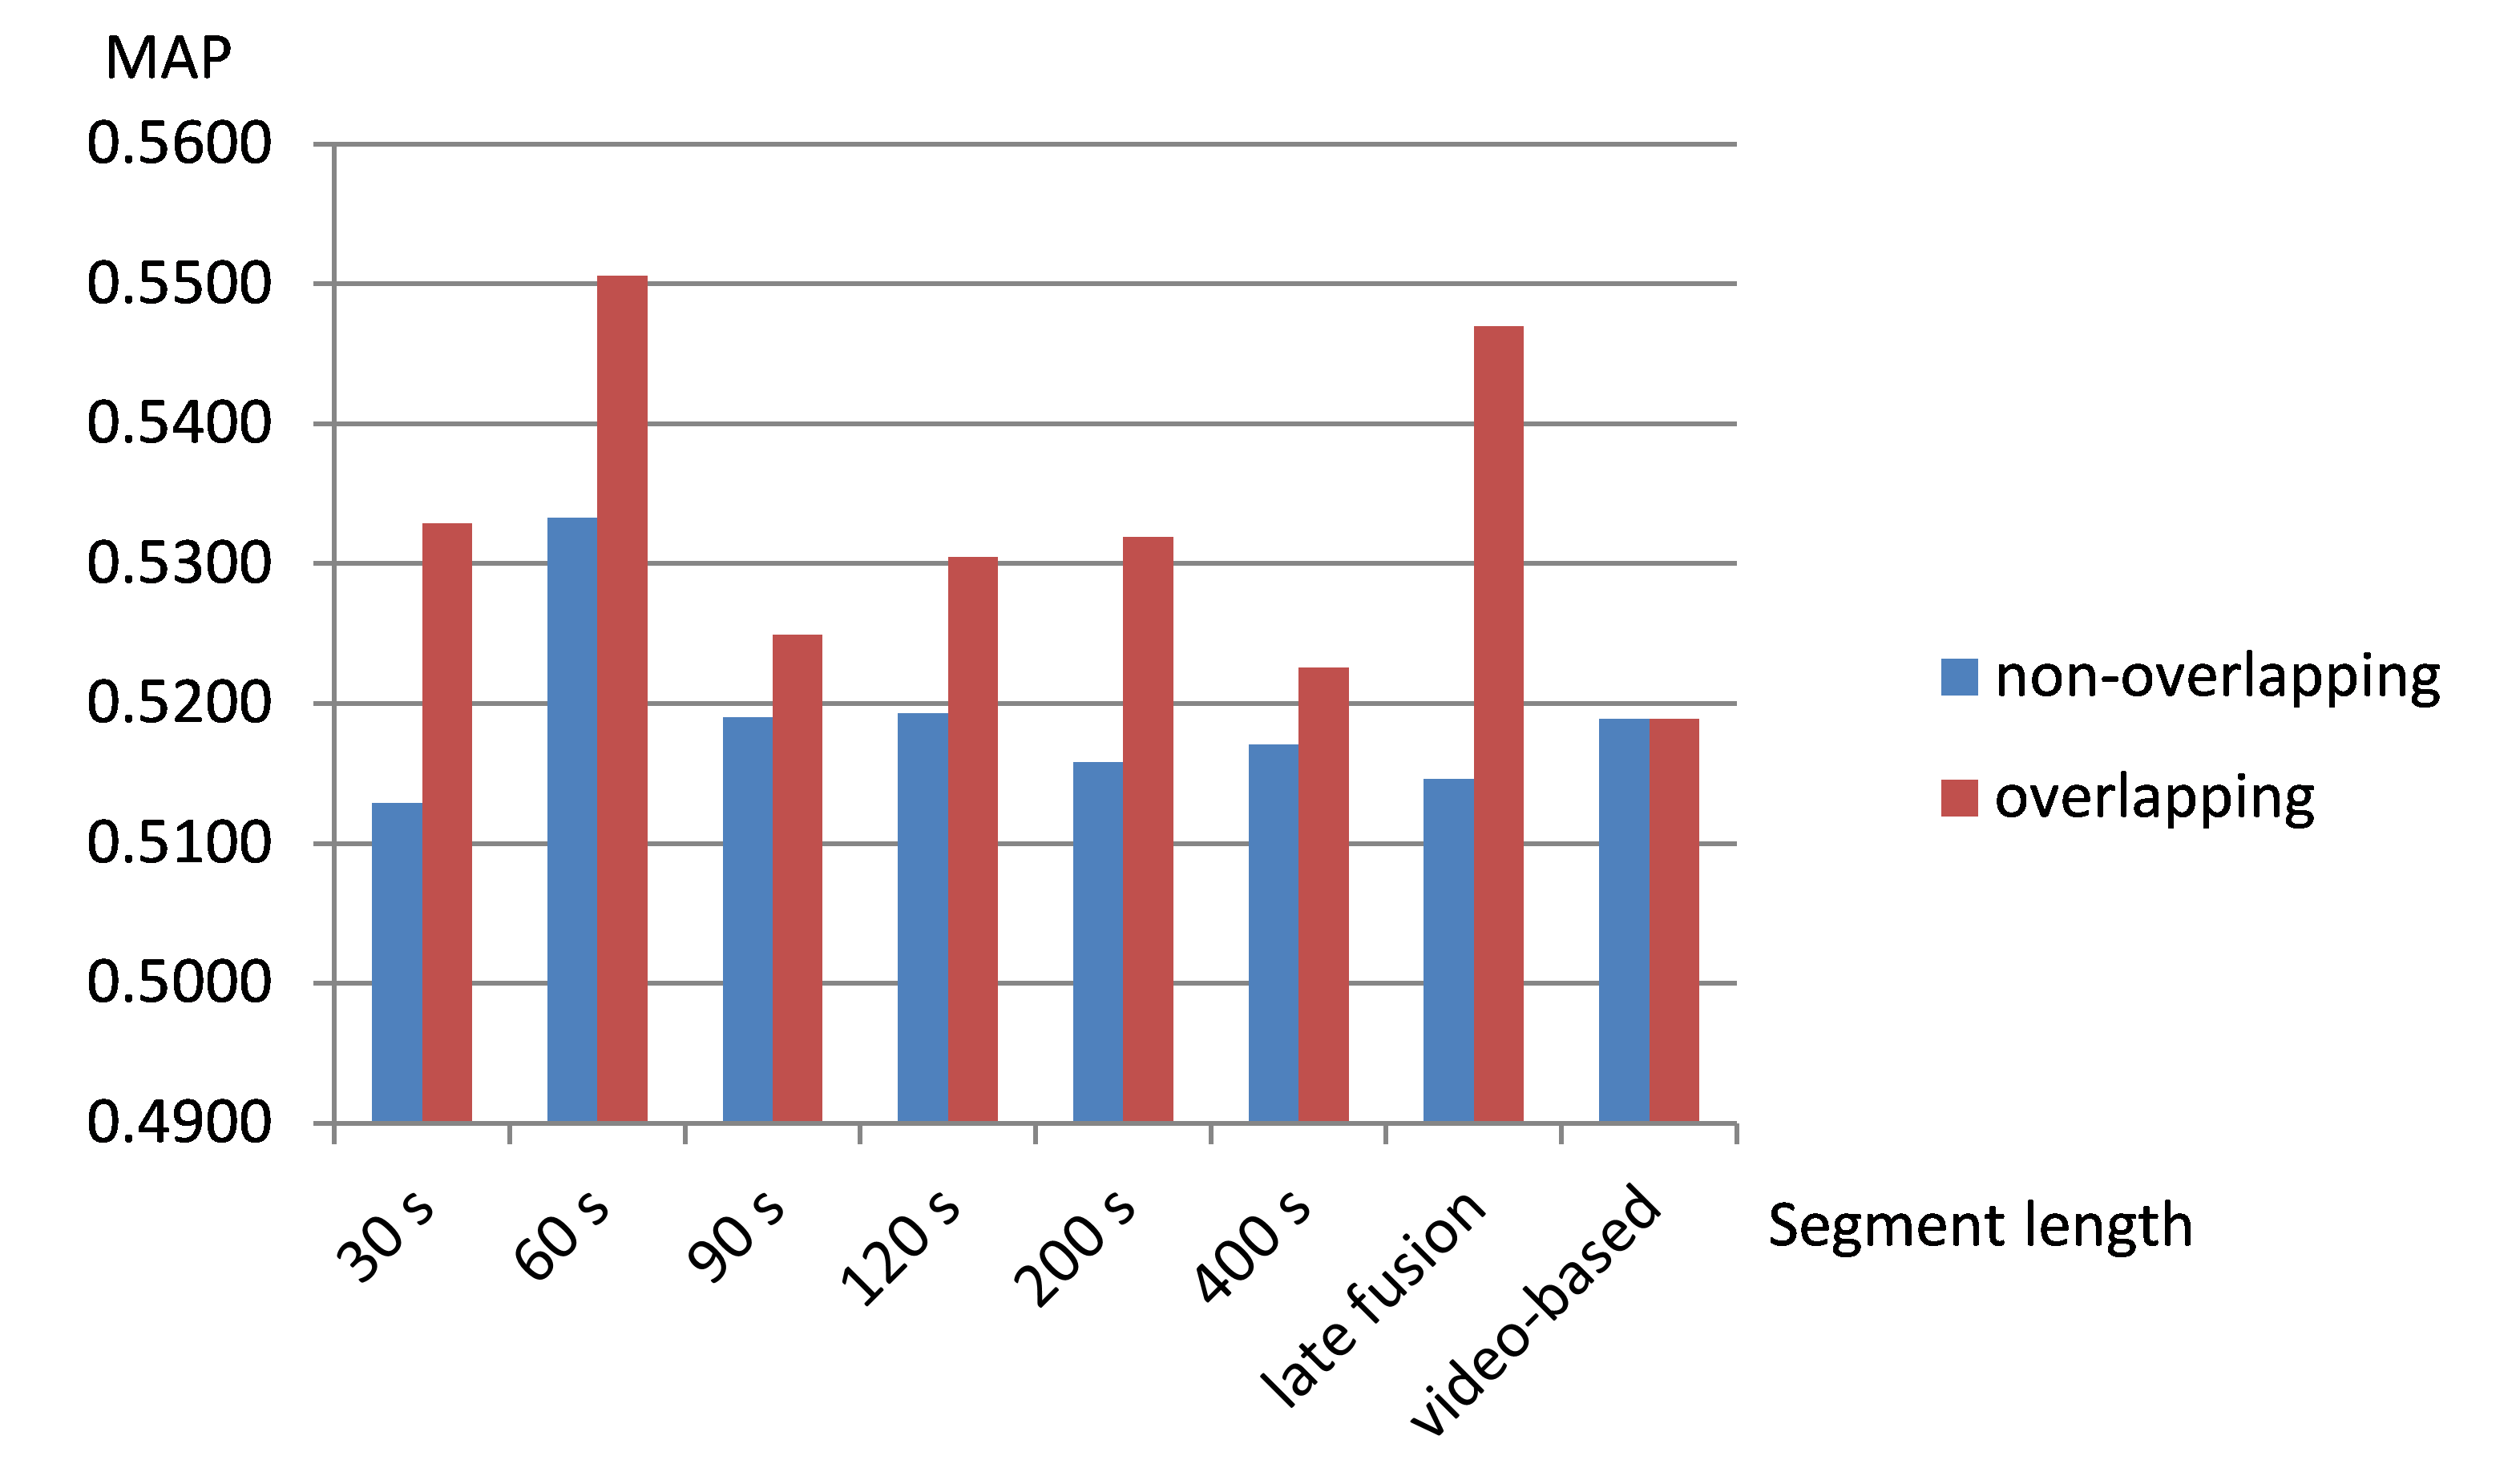
\includegraphics[width=1\textwidth]{med10_result.eps}
	\caption{Results from using segment-based approach with non-overlapping and overlapping sampling on MED 2010. In all cases, the overlapping sampling performs the best}
	\label{f_med10_result}
\end{figure}

\subsection{On TRECVID MED 2010}
\subsubsection{Non-overlapping and overlapping sampling}\label{experimentalresult:1} Table \ref{t_med10_nonoverlapping} lists the results from our segment-based approach when using a non-overlapping sampling strategy. These results show that the performance is rather sensitive to the segment length and it is also event-dependent. For example, the detection results of the first event, ``assembling a shelter'', are better when the segment length is increased. On the other hand, the ``making a cake'' event tends to be more localized, i.e. the shorter the segment, the better the performance. The performance of the ``batting in a run'' event is quite stable when segment length is longer than 60 s. However, it is decreased 2\% at 30 s. This suggests that shorter lengths can harm the performance. In general, the performance of a 60-s segment is the best. This length is also around the geometric mean length of the training set. Thus, we got peak results for segment length around geometric mean point. 

We further investigated the performance of a denser segment sampling, i.e., an overlapping sampling strategy. Interestingly, the MAP score in Table \ref{t_med10_overlapping} is consistently increased for each event compared to the results without using overlapped segments. Figure \ref{f_med10_result} shows a detailed comparison between the two strategies in terms of the over-all performance. We again found that the performance with a segment length around the geometric mean length (60 s) was the best. We also combined the performances of all the segment lengths using late fusion and the results are listed in the last column of Tables \ref{t_med10_nonoverlapping} and \ref{t_med10_overlapping}. The late fusion strategy can benefit the ``making a cake'' event, but it decreased the performances of the remaining events. The overall performance is lower than the best one.
%The performance gain means that denser segment sampling is better. In another words, not only the length of the segment is %important, the location of the segment is also important. This observation lead us to another experiment: using shot boundary %information for choosing segments.

\subsubsection{Segment sampling based on shot boundary detection}
\label{experimentalresult:3}
% For tables use
\begin{table*}
	\renewcommand{\arraystretch}{1.3}
	\caption{Comparison of different segment-based approaches with the video-based approach on the MED 2010 dataset.}
	\label{t_med10_comparison}
	\centering
	% For LaTeX tables use
	\begin{tabular}{|l|ccc|c|c|}
		\toprule
		Event/MAP & \begin{tabular}[x]{@{}c@{}}Best\\non-overlapping\end{tabular}& Best overlapping & SBD segments & Video-based\\
		\midrule
		Assembling shelter & 0.4511 & 0.4781& 0.4284  & \textbf{0.4911} \\
		\midrule
		Batting in a run & 0.7852 &\textbf{0.7918}& 0.7866 & 0.7902 \\
		\midrule
		Making a cake & 0.3636 & \textbf{0.3819} & 0.1918 & 0.2755 \\
		\midrule
		All & 0.5333 & \textbf{0.5506} & 0.4689 & 0.5189 \\
		\bottomrule
	\end{tabular}
\end{table*}

The second column in Table \ref{t_med10_comparison} shows the performance when shot boundary detection is used to extract segments. Unexpectedly, the performance is quite low even when compared with the video-based approach (listed in the last column). There are two possible reasons for this low level of performance: (1) The shot boundary detection technique is inaccurate when used on uncontrolled capturing videos; (2) the shot units may not contain enough information to determine an event. The second reason suggests that combining multiple shots to form a segment may improve the performance. Thus, we have conducted a segment-based experiment based on this observation using segments extracted from multiple shots. However, we did not see any significant improvement. Thus, the first reason is why this experiment had poor result.

We also included the best results from the segment-based experiments using non-overlapping and overlapping sampling in Table \ref{t_med10_comparison} for comparison. In general, our segment-based approach outperforms the video-based approach by more than 3\% in terms of MAP. We did not conduct a keyframe-based experiment because we learned that it is inefficient compared to the video-based approach.

\subsection{On TRECVID MED 2011}

\begin{figure}
	\centering
	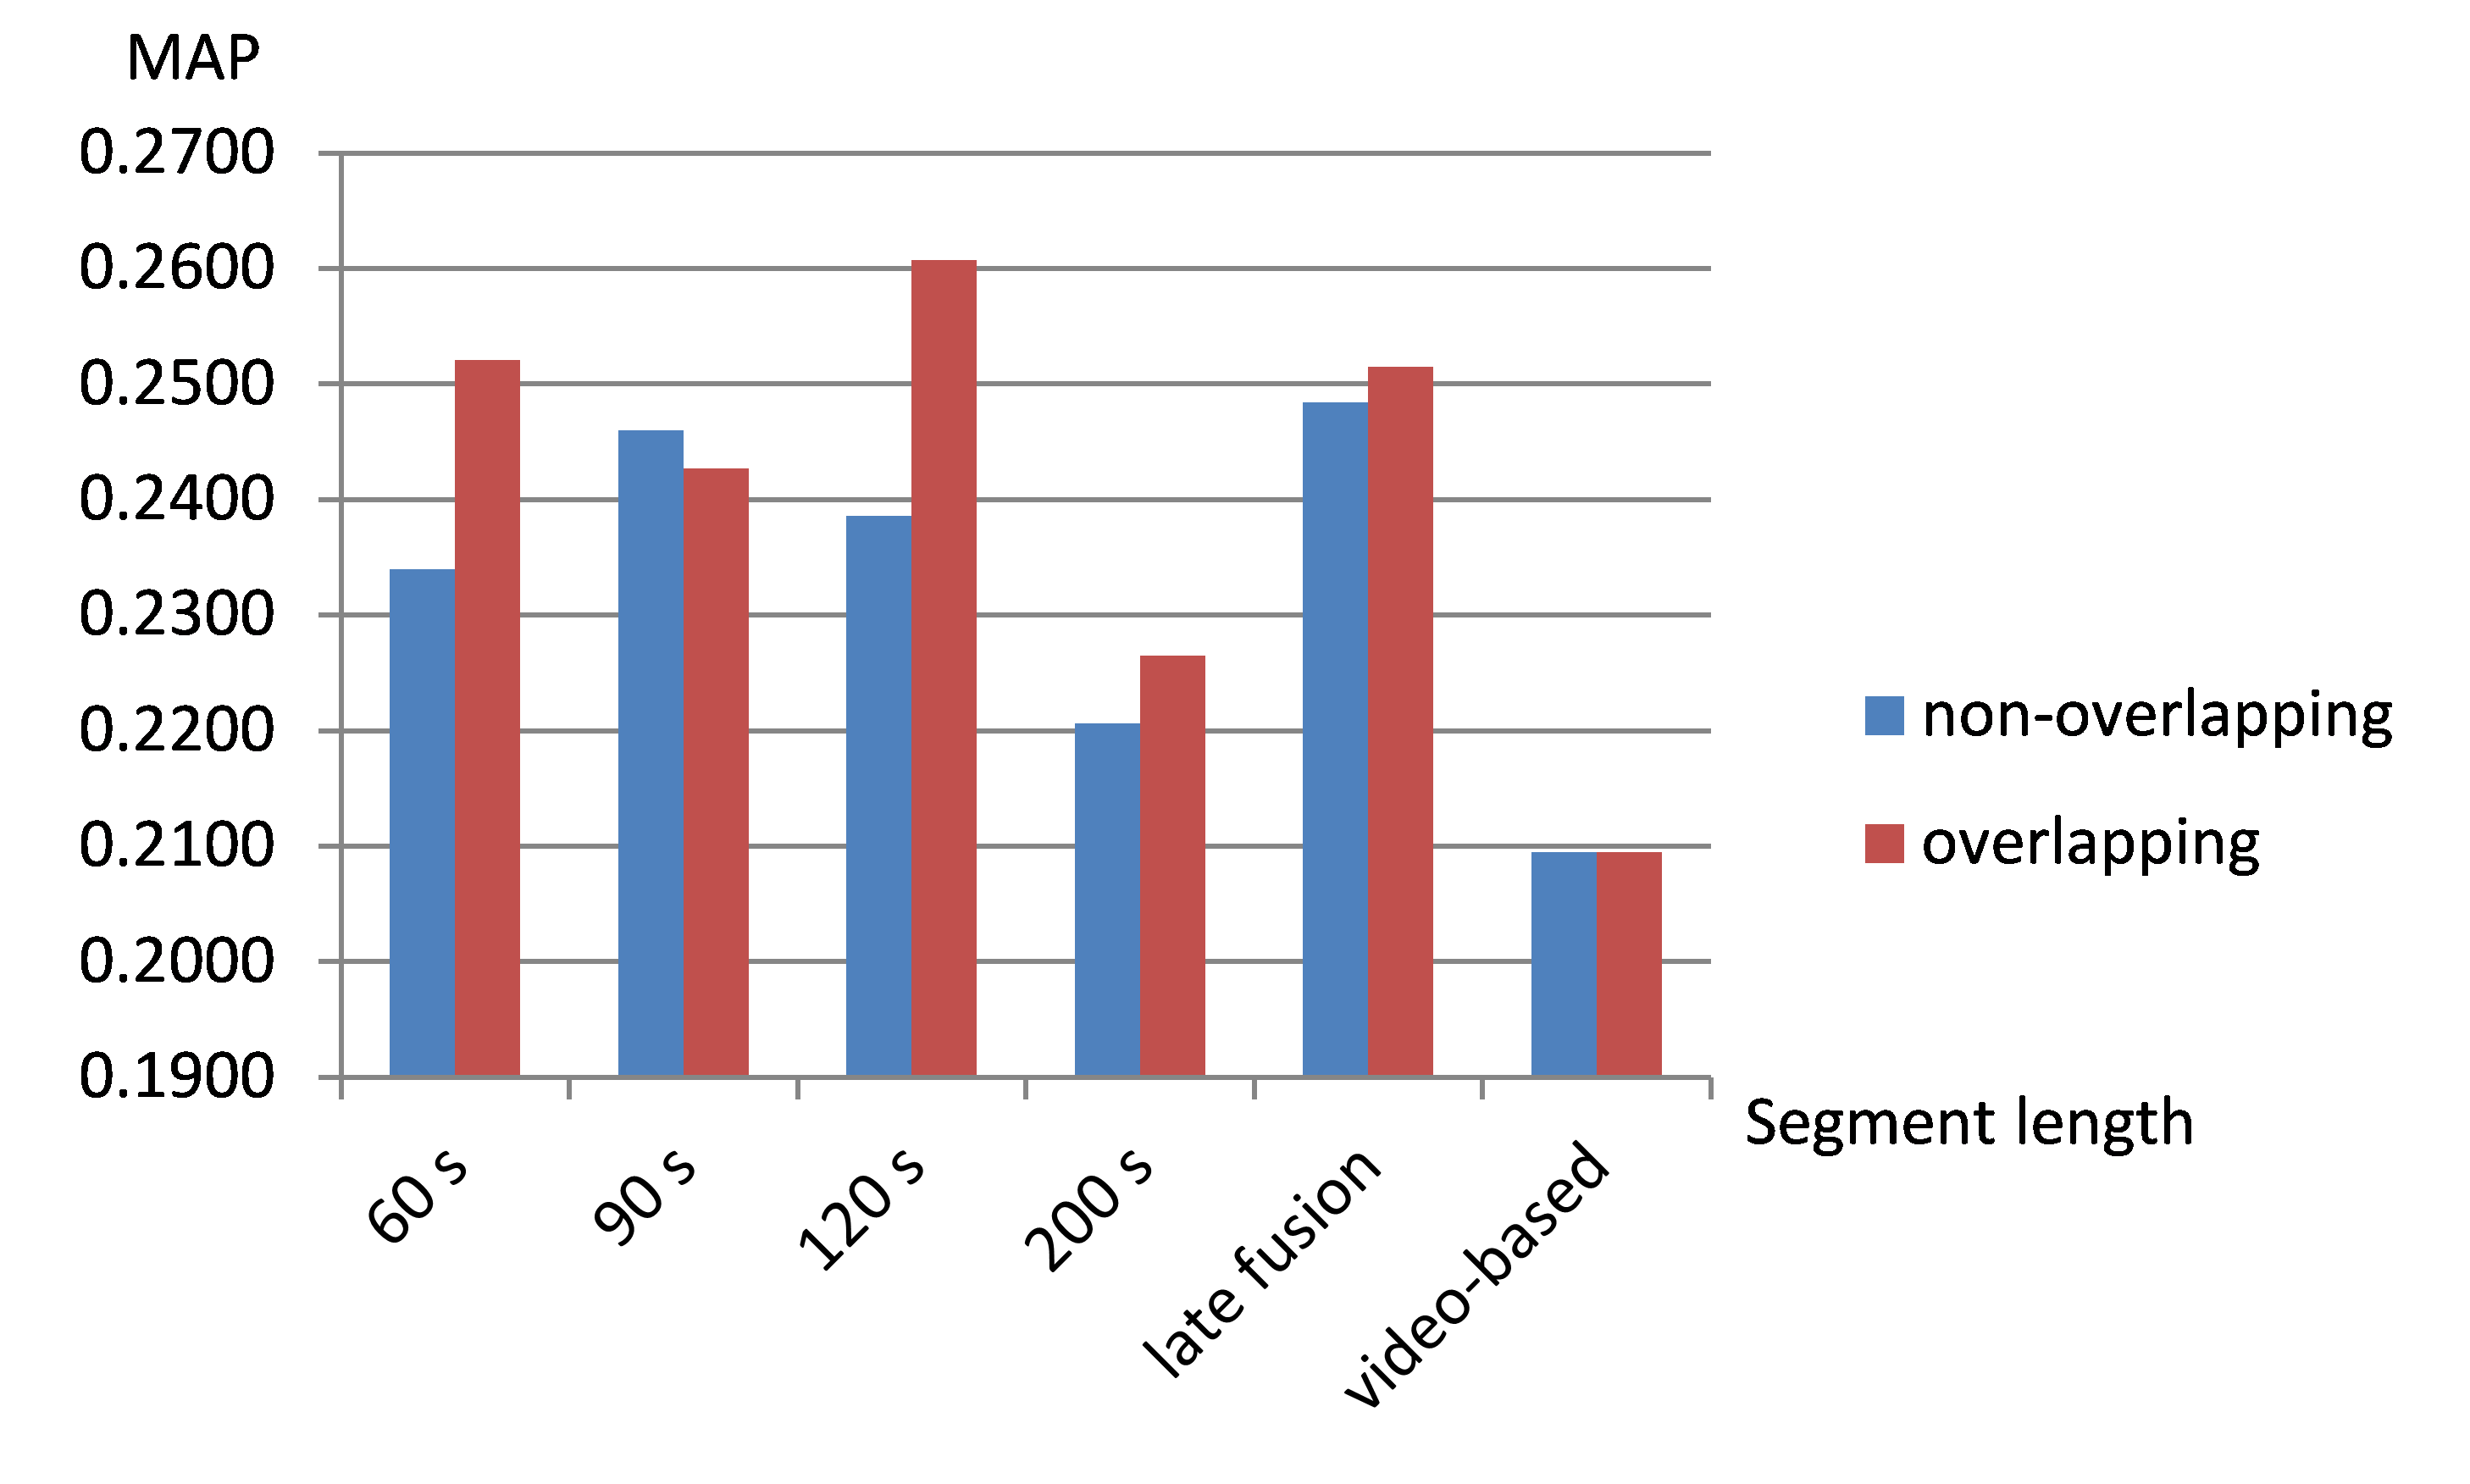
\includegraphics[width=1\textwidth]{med11_result.eps}
	\caption{Results from using segment-based approach with non-overlapping and overlapping sampling on MED 2011. In most cases, the overlapping sampling performs the best.}
	\label{f_med11_result}
\end{figure}

We conducted the same segment-based experiments on MED 2011. For both the non-overlapping and overlapping experiments, we chose segment lengths of 60, 90, 120, and 200 seconds and compare them with the video-based approach. A late fusion strategy is also used to combine the performances of different segment lengths. We did not conduct a shot boundary detection experiment because we showed that it is inefficient. Tables \ref{t_med11_nonoverlapping} and \ref{t_med11_overlapping} list the performances of each event for non-overlapping and overlapping experiment, respectively. Figure \ref{f_med11_result} shows a better view for comparing the overall performance. The result from using video-based approach, which is 0.2095 MAP, is also included for comparison. In most cases, the overlapping sampling had better results than the non-overlapping sampling. In all cases, the segment-based approach also outperforms the video-based approach. The best improvement was about 5\%, which was obtained at 120 s using an overlapping sampling. The late fusion run also confirms its effectiveness for some events, such as ``Flash-mob gathering'' and ``Working on a sewing project''.

% Table generated by Excel2LaTeX from sheet 'new-exp'
\begin{table}[!h]
	\renewcommand{\arraystretch}{1.3}
	\centering
	\caption{Results on the MED 2011 dataset using non-overlapping sampling.}
	\label{t_med11_nonoverlapping}
	\begin{tabular}{|c|c|c|c|c|c|}
		
		\toprule
		\begin{tabular}[x]{@{}c@{}}Event/\\MAP\end{tabular} & 60 s   & 90 s   & 120 s   & 200 s  & \begin{tabular}[x]{@{}c@{}}Late\\fusion\end{tabular} \\
		
		\midrule
		E006&0.1060&\textbf{0.1277}&0.1162&0.1005&0.1217\\
		\midrule
		E007&0.1003&\textbf{0.1521}&0.1461&0.0539&0.1419\\
		\midrule
		E008&0.4811&0.4923&0.4840&0.4508&\textbf{0.4975}\\
		\midrule
		E009&0.2077&0.2072&0.1962&0.1860&\textbf{0.2145}\\
		\midrule
		E010&0.0794&\textbf{0.0916}&0.0486&0.0854&0.0771\\
		\midrule
		E011&\textbf{0.0943}&0.0698&0.0903&0.0703&0.0805\\
		\midrule
		E012&0.3061&0.3560&0.3052&\textbf{0.3639}&0.3309\\
		\midrule
		E013&0.5974&0.6030&0.5861&0.5941&\textbf{0.6033}\\
		\midrule
		E014&0.2307&0.2008&\textbf{0.2772}&0.1723&0.2585\\
		\midrule
		E015&0.1364&\textbf{0.1599}&0.1357&0.1284&0.1583\\
		\midrule
		All&0.2340&0.2460&0.2386&0.2206&\textbf{0.2484}\\
		\bottomrule
		
	\end{tabular}%
\end{table}%

\begin{figure}
	\centering
	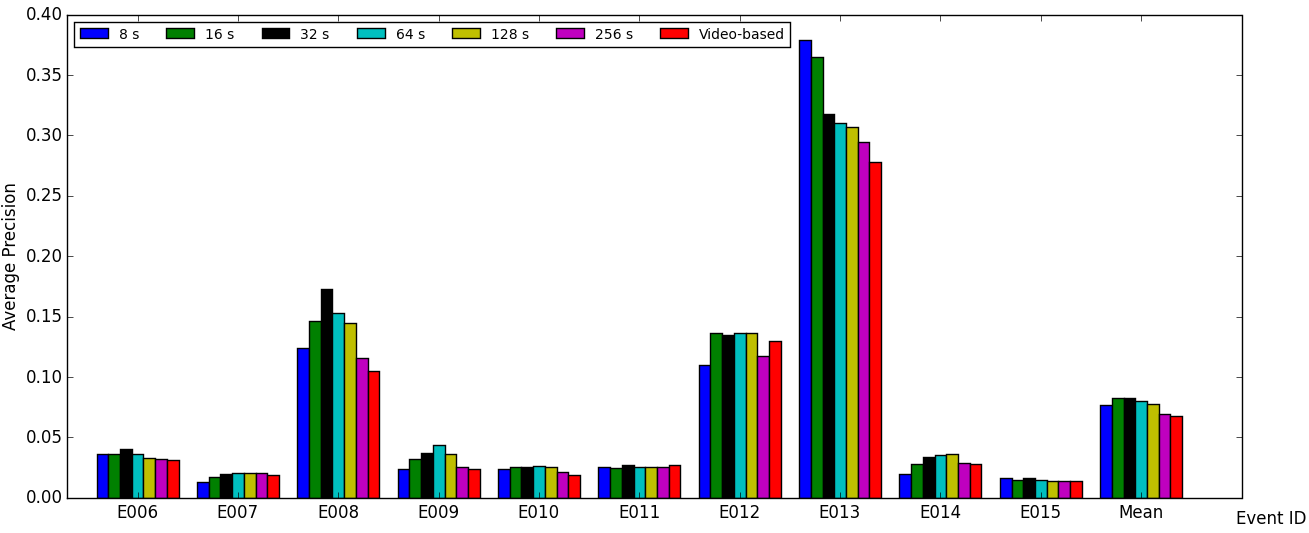
\includegraphics[width=1.1\textwidth]{sb_linear_max.png}
	\caption{Results from using segment-based approach with non-overlapping on the updated MED 2011 dataset.}
	\label{f_med11_update}
\end{figure}

The updated MED 2011 dataset has less number of training videos (See Table \ref{c2_exp_dataset}). We also verify the effectiveness of our approach on this dataset. We conduct experiments at different segment lengths including  8 s, 16 s, 32 s, 64 s, 128 s and 256 s. The overall performance is shown in the last group of Fig. \ref{f_med11_update}.

% Table generated by Excel2LaTeX from sheet 'new-exp'
\begin{table}[!h]
	\renewcommand{\arraystretch}{1.3}
	\centering
	\caption{Results on the MED 2011 dataset using overlapping sampling.}
	\label{t_med11_overlapping}  
	\begin{tabular}{|c|c|c|c|c|c|}
		
		\toprule
		\begin{tabular}[x]{@{}c@{}}Event/\\MAP\end{tabular} & 60 s   & 90 s   & 120 s   & 200 s  & \begin{tabular}[x]{@{}c@{}}Late\\fusion\end{tabular} \\
		
		\midrule  
		E006  & 0.1074 & 0.1069 & \textbf{0.115}1 & 0.1010 & 0.1086  \\
		\midrule  
		E007  & 0.1570 & \textbf{0.1733} & 0.1552 & 0.1466 & 0.1610 \\
		\midrule  
		E008  & 0.4788 & 0.4767 & 0.4969 & 0.4620 & \textbf{0.4903}\\
		\midrule  
		E009  & 0.1830 & 0.1999 & \textbf{0.2160} & 0.1972 & 0.1954 \\
		\midrule  
		E010  & \textbf{0.1150} & 0.0851 & 0.1008 & 0.0746 & 0.1108 \\
		\midrule  
		E011  & 0.0602 & 0.0885 & \textbf{0.1591} & 0.0779 & 0.0819\\
		\midrule  
		E012  & \textbf{0.3674} & 0.3129 & 0.3150 & 0.3075 & 0.3293\\
		\midrule  
		E013  & 0.6025 & 0.5893 & \textbf{0.6188} & 0.5675 & 0.5872\\
		\midrule  
		E014  & 0.2718 & 0.2487 & \textbf{0.2744} & 0.2095 & 0.2706\\
		\midrule  
		E015  & 0.1777 & 0.1459 & 0.1562 & 0.1214 & \textbf{0.1795} \\
		\midrule  
		All   & 0.2521 & 0.2427 & \textbf{0.2607} & 0.2265 & 0.2515 \\
		\bottomrule    
		
	\end{tabular}%
\end{table}%



\section{Discussion}
\label{discussion}
\subsection{Optimal Segment Length} 
It is true that the lengths of the event segments are quite different, even for the same events. Therefore, the fixed length video segments are obviously not the optimal solution to describe the events. However, compared to the video-based approach, as shown in our experiments on the datasets of TRECVID MED 2010 and TRECVID MED 2011, the segment-based approach using overlapping strategy for extracting segments consistently outperforms.

It is ideal if the boundary of the event segment can be determined. However, this localization problem is difficult. The straightforward way to tackle this problem is extracting segments based on shot boundary information. This solution is reasonable because the event might be localized in certain shots. However, we obtained unexpected results due to the unreliability of shot boundary detection in uncontrolled video dataset and the event segment might span to several shots.

The method described in \cite{DBLP:conf/eccv/JiangYY12} suggests another approach to divide a video into segments. Instead of learning a randomized spatial partition for images, we can learn a randomized temporal partition for videos. However, this approach needs sufficient positive training samples while MED datasets have a small number of positive samples with large variation. On the other hand, it is also not scalable because learning and testing the best randomized pattern is time-consuming. Therefore, the fixed-length approach is quite simple but still effective.

Supposed the segment length is fixed, what is the optimal segment length for event detection? This is a difficult question and the answer depends on the dataset. The results of late fusion are quite close to the peak performance of each experiment. This suggests a methodical way to choose the optimal segment length, i.e., combining multiple lengths together (which is similar to \cite{DBLP:conf/eccv/JiangYY12}). However, to achieve the scalability, we should reduce the number of combined lengths as much as possible. From the experimental results on both the MED 2010 and MED 2011 dataset, we observed that with segment length from 60 s to 120 s, the performance is rather stable and close to the peak result. Interestingly, this range is approximate to the range from the geometric mean length to (arithmetic) mean length of the training sets. We also combined multiple segment lengths together using late fusion with equal weights for all segment lengths for comparison. There are two combined runs: one for segment lengths from 60 s to 120 s and the other is for all segment lengths. The result obtained when combining segment lengths from 60 s to 120 s is equivalent to the result obtained when combining all lengths, as shown in Table \ref{t_med11_comparison}. Therefore, based on this observation, we can choose the first combined run as an efficient way for solving the optimal segment length problem of the proposed segment-based approach on other datasets.

\begin{table*}
	\renewcommand{\arraystretch}{1.3}
	\newcolumntype{H}{>{\setbox0=\hbox\bgroup}c<{\egroup}@{}}
	\caption{Comparison of different segment-based approaches with the video-based approach on the MED 2011 dataset.}
	\label{t_med11_comparison}
	\centering
	\begin{tabular}{|c|c|c|c|c|}
		\hline
		\multirow{3}[4]{*}{Event/MAP} & \multicolumn{3}{|c|}{Non-overlapping sampling} &  \multirow{3}[4]{*}{Video-based} \\ 
		\cline{2-4}
		& \begin{tabular}[x]{@{}c@{}}Best\\(at 90 s) \end{tabular}
		& \begin{tabular}[x]{@{}c@{}}Late fusion\\(all lengths) \end{tabular}
		& \begin{tabular}[x]{@{}c@{}}Late fusion\\(60, 90, 120 s) \end{tabular} & \\ \hline
		
		E006  & \multicolumn{1}{|c|}{\textbf{0.1277}} & 0.1217 & 0.1244 & 0.0959 \\ \hline
		
		E007  & \multicolumn{1}{|c|}{0.1521} & 0.1419 & \multicolumn{1}{|c|}{0.1369} & 0.1303 \\	\hline
		E008  & \multicolumn{1}{|c|}{0.4923} & \textbf{0.4975} & \multicolumn{1}{|c|}{0.4973} & 0.4766 \\	\hline
		E009  & \multicolumn{1}{|c|}{0.2072} & 0.2145 & \multicolumn{1}{|c|}{0.2064} & 0.0943 \\	\hline
		E010  & \multicolumn{1}{|c|}{0.0916} & 0.0771 & \multicolumn{1}{|c|}{0.0753} & 0.1020 \\	\hline
		E011  & \multicolumn{1}{|c|}{0.0698} & 0.0805 & \multicolumn{1}{|c|}{0.0813} & 0.0609 \\	\hline
		E012  & \multicolumn{1}{|c|}{\textbf{0.3560}} & 0.3309 & \multicolumn{1}{|c|}{0.3277} & 0.2858 \\	\hline
		E013  & \multicolumn{1}{|c|}{0.6030} & 0.6033 & \multicolumn{1}{|c|}{0.6096} & 0.5385 \\	\hline
		E014  & \multicolumn{1}{|c|}{0.2008} & 0.2585 & \multicolumn{1}{|c|}{0.2579} & 0.2138 \\	\hline
		E015  & \multicolumn{1}{|c|}{0.1599} & 0.1583 & \multicolumn{1}{|c|}{0.1622} & 0.0964 \\	\hline
		All   & \multicolumn{1}{|c|}{0.2460} & 0.2484 & \multicolumn{1}{|c|}{0.2479} & 0.2095 \\	\hline
		
	\end{tabular}%
	\label{tab:addlabel}%
\end{table*}%



\begin{table*}
	\renewcommand{\arraystretch}{1.3}
	\caption{Comparison of different segment-based approaches with the video-based approach on the MED 2011 dataset.}
	\label{t_med11_comparison}
	\centering
	\begin{tabular}{|c|c|c|c|c|}
		\toprule
		\multirow{3}[4]{*}{Event/MAP} & 
		 \multicolumn{3}{|c|}{Overlapping sampling} & \multirow{3}[4]{*}{Video-based} \\ 
		\cline{2-4}
		& \begin{tabular}[x]{@{}c@{}}Best\\(at 120 s) \end{tabular}
		& \begin{tabular}[x]{@{}c@{}}Late fusion\\(all lengths) \end{tabular}
		& \begin{tabular}[x]{@{}c@{}}Late fusion\\(60, 90, 120 s) \end{tabular} &  \\ \midrule
		E006  & 0.1151 & 0.1086 & \multicolumn{1}{|c|}{0.1083} & 0.0959 \\ \midrule
		
		E007  & 0.1552 & 0.1610 & \multicolumn{1}{|c|}{\textbf{0.1616}} & 0.1303 \\	\midrule
		E008  & 0.4969 & 0.4903 & \multicolumn{1}{|c|}{0.4871} & 0.4766 \\	\midrule
		E009  & \textbf{0.2160} & 0.1954 & \multicolumn{1}{|c|}{0.1958} & 0.0943 \\	\midrule
		E010  & 0.1008 & 0.1108 & \multicolumn{1}{|c|}{\textbf{0.1109}} & 0.1020 \\	\midrule
		E011  & \textbf{0.1591} & 0.0819 & \multicolumn{1}{|c|}{0.0845} & 0.0609 \\	\midrule
		E012  & 0.3150 & 0.3293 & \multicolumn{1}{|c|}{0.3341} & 0.2858 \\	\midrule
		E013  & \textbf{0.6188} & 0.5872 & \multicolumn{1}{|c|}{0.5910} & 0.5385 \\	\midrule
		E014  & \textbf{0.2744} & 0.2706 & \multicolumn{1}{|c|}{0.2694} & 0.2138 \\	\midrule
		E015  & 0.1562 & 0.1795 & \multicolumn{1}{|c|}{\textbf{0.1795}} & 0.0964 \\	\midrule
		All   & \textbf{0.2607} & 0.2515 & \multicolumn{1}{|c|}{0.2522} & 0.2095 \\	\bottomrule
		
	\end{tabular}%
	\label{tab:addlabel2}%
\end{table*}%

\subsection{Scalability} For scalability, we discuss the storage and computation costs of our experiments. At first, our system does not consume a lot of disk storage because we only store the final representation of the videos or segments, not the raw features. We calculated the BoW features directly from the raw feature outputs using a pipeline reading technique. One drawback is that this technique requires a lot of memories. However, we handled this problem by encoding the raw features into smaller chunks and aggregating them to generate the final representation. By this way, we can manage the mount of memory usage.

In our framework, the most time-consuming steps are the feature extraction and representation (using the bag-of-words model). It is worth noting that the computation time for one video is independent of the segment length, which means our segment-based approach has the same computational cost as the video-based approach. On the other hand, when we do experiments at the segment level, we will have more training and testing samples than that in the video-based approach. Thus, it will cost more in time to train and test using the segment-based approach. However, this cost is relatively small compared with the feature extraction and representation cost. For example, when using a grid computer with 252 cores, it took us about 10 hours to generate the feature representation for each segment-based experiment on MED 2010 dataset. In the mean time, we used one-core processor for the training and testing, but it only took about 4-8 hours for the training and 2-4 hours for the testing on each event. For the MED 2011 dataset, the computational cost was around 13 times bigger than the MED 2010 (linearly to the number of videos it contains).

\section{Conclusion}
\label{c3_conclusion}
We proposed using the segment-based approach for multimedia event detection in this work. We evaluated our approach by using the state-of-the-art dense trajectories motion feature on the TRECVID MED 2010 and TRECVID MED 2011 datasets. Our proposed segment-based approach outperforms the video-based approach in most cases when using a simple non-overlapping sampling strategy. More interestingly, the results are significantly improved when we using the segment-based approach with an overlapping sampling strategy. Therefore, the effectiveness of our methods on realistic datasets like MEDs is confirmed.

A segment-based approach with an overlapping sampling strategy shows promising results. This suggests the importance of segment localization on the MED performance. Suppose the segment length is fixed, we are interested in determining which segment is the best representative for an event. In this study, we also observed that the detection performance is quite sensitive to the segment-length and it depends on the dataset. The results obtained from the late fusion strategy is quite stable and close the peak performance. This suggests a methodical way to generalize the segment-based approach to other datasets. However, this method is not scalable because it requires a lot of computation costs. Therefore, learning an optimal segment length for each event can be beneficial for an event detection system. This is also an interesting direction for our future study.

